\documentclass[APA,STIX1COL]{WileyNJD-v2}

\articletype{Article Type}%

\received{26 April 2016}
\revised{6 June 2016}
\accepted{6 June 2016}

\raggedbottom

\begin{document}

\title{Multiple change point detection  on air pollution via genetic algorithms with bayesian-MDL on nonhomogeneous Poisson periods.}


\author[1]{Arrigo Coen*}

\author[2,3]{Biviana Su\'arez Sierra}

\author[3]{J. Fernando Castillo}

\authormark{AUTHOR ONE \textsc{et al}}


\address[1]{\orgdiv{Org Division}, \orgname{Org Name}, \orgaddress{\state{State name}, \country{Country name}}}

\address[2]{\orgdiv{Org Division}, \orgname{Org Name}, \orgaddress{\state{State name}, \country{Country name}}}

\address[3]{\orgdiv{Org Division}, \orgname{Org Name}, \orgaddress{\state{State name}, \country{Country name}}}

\corres{*Corresponding author name, This is sample corresponding address. \email{authorone@gmail.com}}

\presentaddress{This is sample for present address text this is sample for present address text}

\abstract[Summary]{
It is well documented that the presence of high amounts of particulate exceedances has adverse effects on human health and damages the equilibrium of ecosystems. To reduce air pollution, governments modify public enviromental policies. One method to find out if a new  policy has a positive effect is to examine if a change in the probabilistic behavior of the environmental markes happen after the implementation of a new policy. In this study, we model the number of particulate exceedances with a nonhomogeneous Poisson process and implement a genetic algorithm to search for  change points  in its complex structure. We applied our model to analyze data from january  2018 to december 2020 of Bogota, Colombia and found a relationship between the new public polices and the occurrences of change points.}

\keywords{MDL, genetic algorithm, Nonhomogenous Poisson, air pollution, PM2.5}


\jnlcitation{\cname{%
\author{A. Coen}, 
\author{M. Su\'arez Sierra}, 
\author{J.F. Castillo}}} (\cyear{2021}), 
\ctitle{Multiple changepoint detection on air pollution via genetic algorithms with bayesian-MDL on nonhomogeneous Poisson periods}, \cjournal{Envirometrics}, \cvol{2021.}

\maketitle


\section{General Comments}\label{sec1}


In the present article we determine the points of change in the data of exceedances of $PM_{2.5}$ from January 2018 to December 31 2020 in Bogot\'a, Colombia. The way in which the points of change and their respective locactions are established, is by means of the genectic algorithm, which is based on the interaction of two chromosomes (mother and father). to conceive a generation of descendants with certain suitable facets to be a well-qualified candidate through the MDL (minimum length of description). For the purposes of the implementation of the generic algorithm to change points, each of the $\binom{N}{m}$ configuration options has the form $(m,\tau_1,\tau_2,...,\tau_m)$, where $m$ is the number of  points of change, $\tau_i$ is the location of the point of change $i$, with $i=1, .. , m$, $\tau_i=2, ..., N-1 $. In the generic algorithm at each configuration $(m, \tau_1, \tau_2, ..., \tau_m)$ is called a chromosome. Data from Bogota were used with N = 1096, , which is the number of days in three years of observation.  with special emphasis on the days in which the limit established by the regulations (37 $\mu/m^3$) is exceeded, in order to establish when there is an acute increase or decrease.  


\section{Introduction}\label{sec2}

Air pollution is one of the greatest public health threats of our times, and in recent years several links have been found between various health problems and poor air quality. 
Several studies such as \cite{Janssen}, have shown that permanent exposure to particulate matter $PM_{2.5}$ (particulate matter with a diameter of less than 2.5 micrometers or microns ($\mu m$)) is related to a decrease in life expectancy as it increases the risk of lung cancer, cardiovascular and pulmonary diseases.\\

This is no small matter, in October 2013 the World Health Organization (WHO), more precisely ,\cite{IARC} reported that there is abundant evidence that air pollution can be considered as a carcinogenic agent for humans. In addition to the cancer and health effects already mentioned, of special importance is the effect that air pollution has on pregnant women, \cite{Keplac}, \cite{Laurent},\cite{Xiao}
It has been shown that there is a relationship between high levels of PM 2.5 and adverse pregnancy outcomes, This  can be explained due to the fact that pregnancy may constitute a state particularly susceptible to toxins contained in air pollution because of high level of cell proliferation, organ development and the changing capabilities of fetal metabolism. PTB (Preterm Birth) and LBW (Low Birth Weight) are the most frequently investigated outcomes. Poor air quality also generates health effects beyond those normally expected; recently a connection has been found between poor air quality and an increase in risk factors for type 2 diabetes, \cite{Thiering}, \cite{Lim} The cumulative evidence seems to indicate a positive association between short-term and long-term air pollution exposure and the mortality risk in diabetic subjects. In addition, most of these studies reported a greater PM-associated mortality risk in diabetic patients than in the non-diabetic populations.

Besides  the negative effects on human health, air pollution also causes damage to ecosystems, the emission of NOx, SOx and PM contributes to an accumulation of nitrogen and sulfur in the environment that creates an alteration in the biochemistry of terrestrial, wetland and aquatic ecosystems. This accumulation alters the biogeochemistry and the physiology of organisms, resulting in harmful declines in biodiversity. In addition to the loss of unique living species, the decline in total biodiversity is harmful because biodiversity is an important determinant of the stability of ecosystems and the ability of ecosystems to provide services to humanity. New research confirms that nitrogen and sulfur deposition causes acidification of terrestrial ecosystems, leading to a decrease in lichen and herb/forb biodiversity and changes in soil chemistry, as consequence the ability of plant roots to take up base cations (especially calcium [Ca]) and water from the soil is decreased. Effects on the soil and the acidifying deposition on foliage can influence the response of plants to climatic stresses such as drought and cold temperature. The effects of acidifying deposition can also influence the sensitivity of plants to other stresses, including insect pests and disease.\cite{EPA}

In Latin America, Mexico City and Bogota are among the cities with the highest rates of air pollution, which would imply a deterioration of public health in different aspects, as well as damage to the ecosystems of these cities.
This pollution has  consequences in the inhabitants of the city,  according to the INS (National Health Institute), the healthcare provider institutions registered 1.732.375 individuals consulting for respiratory disease in  2017. \cite{INS} The INS suggests that children under the age of 1 have been most affected by their immature respiratory system and individuals over the age of 60 may be affected by this age due to the weakening of their health.  

For these reason, these cities have been implementing air quality measurement stations. We believe it is important to find the points of change in the measurements obtained, to determine when they occur and if these changes are due to decisions taken by the authorities, and likewise if these actions do not generate a change in the behavior of air pollution. 

In practice, there is no information about the change points of a time series, no knowledge of when they occur, and no knowledge of how many there are. The objective of this article is to find the change points in the measurements of $PM_{2.5}$ in the city of Bogota. This problem is therefore approached as one of optimization of an objective function over all possible change points and their positions. Since it is not computationally optimal to search for all possible configurations of change points, it is optimized by a genetic algorithm that runs through a subset of good models and intelligently selects the best one according to a given criterion.



First, two methods are described for parameter estimation in the presence of an inhomogeneous Poisson process, which is determined by its intensity function. In the first method, the parameter settings include change points, which mark in a time series the transition from one behavioral regime to another. This time series will be daily ozone or $PM_{2.5}$ measurements of the air of some selected city. Secondly, we show an estimation technique for the change points, these will constitute a vector called chromosome. In addition to the information on the location of the change points, the first entry of the chromosome will indicate how many change points are suggested in the time series studied. 


Our proposal is a combination of these two methodologies, the first one was used to estimate the different parameters of the non-homogeneous Poission distribution and the second methodology was used to estimate the amount and location of the change points of the ozone time series in Bogota between 2018 and 2020


\section{Bogotá Pollution DataSet}\label{sec3}

Since $1982$ was established in Colombia the regulations regarding air quality, this legislation has been updated over time to adjust for the changing needs of the country. The last change was made in Resolution 2254 of 2017 of the Ministry of Environment and Sustainable Development. In it it was established that the standard pollutants are $PM_{10}$, $PM_{2,5}$, $SO_2$, $CO$, $NO_2$ and $O_3$. Previously the local governmental established the maximum allowable concentration level for each of the pollutants; for $PM_{10}$ it is $75 \mu g m^3$, $PM_{2,5}$ is $37 \mu g m^3$ and ozone is $80 \mu g m^3$. \cite{decenal}

Consistent with these directives of the Minister of Environment and Sustainable Development, in 2018 the document CONPES 3943  established a policy aimed at reducing the concentration of these pollutants. For this purpose, action plans were established that aim to renew the public service and cargo transportation vehicles, reduce the sulphur content of fuels (mobile sources), and implement better techniques and industrial practices (stationary sources) (DNP, 2018).In order to make this a success, different government institutions such as the Ministry of Environment and Sustainable Development, the Ministry of Health and Social Protection and the Institute of Hydrology, Meteorology and Environmental Studies (IDEAM) have to work in conjunction with each other.

In addition to national guidelines and plans, since 1991, Bogota through the Mayor's Office and the city's Secretary of the Environment have issued resolutions that aim to ensure air quality. For example, the District Environment Secretariat can declare (and finish) environmental emergencies (Resolution 632 of 2019), for example when thresholds established in the IBOCA (Bogota Air Quality and Health Risk Index) are exceeded. Also, the Mayor's Office of Bogota has adopted some restrictions on the hours and days that vehicles can transit in the city, this to reduce air pollution in the city (Decree 174 of 2006).

The Mayor's Office of Bogota developed a strategy that aims to coordinate the actions of the protagonists responsible for decontaminating the air, preventing and reducing the impacts of pollution on the citizens of the city and its environment, this strategy is called the Ten-Year Plan for Air Decontamination 2010-2020. The plan identified that the main pollution problem in Bogota is particulate matter ($PM_{2.5}$ and $PM_{10}$).  The plan also calculated the Percentage Index of Excesses (IPE), based on \cite{Gaitan}, which compares the RMCAB data with air quality regulations.  This serves as a reference to see the level of compliance with criteria pollutants. It was found that on average, in 2010, 40\% of the days of the year, the $PM_{10}$ exceeded the annual standard. The percentage of non-compliance for the remaining pollutants was less than 5\% (Alcaldía de Bogotá 2010).

To collect information on the levels of air pollution in the city, the district has the Bogotá Air Quality Monitoring Network - RMCAB, consisting of 13 fixed monitoring stations and one mobile station, which are located in different parts of the city.
This network reported that in three of the first four months of 2019 pollution levels for $PM_{2,5}$ were above the maximum permissible standard, ($37 \mu g / m$). This indicates that the high levels of this pollutant is a problem for Bogota and that the quality of the policies taken by the mayor's office should be evaluated.
To find the number of change points and their position in the $PM_{2,5}$ time series in Bogota, models used in Mexico City were studied, the following section will explain how these models were constructed.


\section{INFERENTIAL ANALYSIS OF THE UNIVARIATE NON-HOMOGENEOUS POISSON
PROCESS}\label{sec4}



Several studies have been conducted on air quality in Mexico City, including some that make use of stochastic models, in order to make statistical inferences about the behaviour of some air quality characteristics.In particular, \cite{Achcar09} and \cite{Achcar10} investigated the distribution of the number of times that the maximum daily ozone levels in Mexico City exceed the environmental standard or some environmental thresholds. Considering the regulations of the City of Mexico and the country in general, a threshold of $0.17$ parts per million (ppm) was chosen as this was an intermediate value between the meridian environmental standard at the time, $0.11$ ppm of and the threshold of $0.2$ ppm established to declare environmental emergencies in the City of Mexico. In these two papers, three possible parametric forms for the intensity function $\lambda(t)$ are considered. In \cite{Rodrigues13} different forms for the rate function $t\geq 0$ can be observed.
To find this distribution, Poisson models are used,it is assumed that that the rate of the Poisson process changes with time, which is reflected in the parameters of the Poisson distribution, 

These special cases of functions were used to model the  intensity function, which describes the ozone pollution data in Mexico City: Weibull (W) [\cite{Govind95}, \cite{Cid99}], Musa-Okumoto (MO)[\cite{Musa84}], Goel-Okumoto (GO) [\cite{Goel78}] and a generalization of the Goel-Okumoto model (GGO), for which the $m(t|\mathbf{\theta})$ is defined respectively by:
\begin{eqnarray}
	\label{eq1}
	\begin{array}{llll}
		m^{(W)}(t|\mathbf{\theta}) &=& (t/\beta)^{\alpha}, &\alpha ,\beta >0\\
		m^{(MO)}(t|\mathbf{\theta}) &=& \beta\log \left(1+\frac{t}{\alpha}\right), &\alpha ,\beta >0\\
		m^{(GO)}(t|\mathbf{\theta}) &=& \alpha [1-\exp (-\beta t)], &\alpha ,\beta >0\\
		m^{(GGO)}(t|\mathbf{\theta}) &=& \alpha [1-\exp (-\beta t^\gamma)], &\alpha ,\beta , \gamma >0.\\
	\end{array}
\end{eqnarray}

For the first three cases the vector of parameters is $\theta=(\alpha ,\beta )$ and for the last model $\theta=(\alpha ,\beta, \gamma)$ respectively. The corresponding rate functions $\lambda(t)$, $t\geq 0$ or risk are: 

\begin{eqnarray}
	\label{eq2}
	\begin{array}{llll}
		\lambda^{(W)}(t|\mathbf{\theta}) &=& (\alpha/\beta)(t/\beta)^{\alpha-1}, &\alpha ,\beta >0\\
		\lambda^{(MO)}(t|\mathbf{\theta}) &=& \frac{\beta}{t+\alpha}, &\alpha ,\beta >0\\
		\lambda^{(GO)}(t|\mathbf{\theta}) &=& \alpha\beta\exp (-\beta t), &\alpha ,\beta >0\\
		\lambda^{(GGO)}(t|\mathbf{\theta}) &=& \alpha\beta\gamma t^{\gamma-1}\exp (-\beta t^\gamma), &\alpha ,\beta , \gamma >0.\\
	\end{array}
\end{eqnarray}

Furthermore, in the applications to the Mexico City data, the possibility that the data could change its behaviour over time was considered. This property was studied considering the presence of change points in the non-homogeneous Poisson model.\\ 


\subsection{Likelihood function with change points}

A changepoint is a time where the structural pattern of a time series shifts, we assumed the presence of $J$ time instantes, $\{\tau_1, \tau_2, \cdots ,\tau_J\}$, the points where there are changes in the model parameters, caused by some event such as the effects of a new environmental legislation in a certain year or suspension of the operation of some network station due to maintenance. The intensity functions of the NHPP have the form


\begin{eqnarray}
	\label{eq3}
\lambda(t | \theta) = 
\left\lbrace
\begin{array}{lll}
	\lambda(t|\theta_1), & 0\leq t< \tau_1, &\\
	\lambda(t|\theta_j), & \tau_{j-1}\leq t<\tau_j, & j = 2,3,\cdots,J,\\
	\lambda(t|\theta_{J+1}). &\tau_J\leq t\leq T,  &
\end{array}
\right.
\end{eqnarray}


Where $\theta_j$ is the vector of parameters between the change points $\tau_{j-1}$ and $\tau_j$, $j=2,...,J$, $\theta_1$ and $\theta_{J+1}$ are the parameter vectors before and after the first and last change points, respectively.
With $n$ observations, the functions for the means are [see, e.g., \cite{Rodrigues13}],


\begin{eqnarray}
	\label{eq4}
m(t|\theta) = 
\left\lbrace
\begin{array}{lll}
	m(t|\theta_1), & 0\leq t< \tau_1, &\\
	m(\tau_1|\theta_1) + m(t|\theta_2) - m(\tau_1|\theta_2), & \tau_1\leq t<\tau_2, \\
	m(t|\theta_{j+1}) - m(\tau_j|\theta_{j+1}) \\+ \sum_{i=2}^{j}[m(\tau_i|\theta_i) - m(\tau_{i-1}|\theta_i)] \\+ m(\tau_1|\theta_1),  & \tau_{j}\leq t<\tau_{j+1}, & j = 2,3,\cdots,J.
\end{array}
\right.
\end{eqnarray}


where $\tau_{J+1}=T$. That is, in the present study $m(t|\theta_1)$ represents the average number of exceedances of the standard, before the first change point, since the vector of parameters $\theta_1$ is known;  $m(\tau_1|\theta_1) + m(t|\theta_2)-m(|\tau_1|\theta_2)$ is the average number of exceedances of the standard, between the first change point $\tau_1$ and the second $\tau_2$, given that the vector of parameters $\theta_2$ is known, and so on. \\

%The data set on which the above formulations were made is given by.\\

Let $D={d_1,\ldots ,d_n}$, where $d_k$ (as in the case without change points), is the time of occurrence of the $kth$ event (in the case in which the $kth$ time in which the maximum level of the environmental standard is exceeded), $k=1,2,...,n$.  The likelihood function is determined by the expression below
where $N_{\tau_i}$, represents the number of overpasses before the change point $\tau_i$, with $i=1,2,...,J$. [see, \cite{Yang}, \cite{Achcar11}]


\begin{align}
	\label{eq5}
	L(\mathbf{D}|\phi) \propto &  \left[\prod_{i=1}^{N_{\tau_1}}\lambda(d_i\ | \ \theta_1) \right]e^{-m(\tau_1 | \theta_1)}\nonumber\\
	& \times \left[ \prod_{j=2}^{J} \left( \prod_{i=N_{\tau_{j-1}}+1}^{N_{\tau_j}}\lambda(d_i |\theta_j)\right)e^{-[m(\tau_j |\theta_j)-m(\tau_{j-1} | \theta_j )]}  \right]\nonumber\\
	& \times \left[\prod_{i=N_{\tau_{J}}+1}^{n}\lambda(d_i|\theta_{J+1})\right]e^{-[m(T |\theta_{J+1})-m(\tau_{J}|\theta_{J+1} )]},
\end{align}


Using the expression (\ref{eq5}) we make inference of the parameters $\phi=(\theta, \tau)$ with $\theta=(\theta_1,...,\theta_J)$ and $\tau=(\tau_1,...,\tau_J)$, using the Bayesian approach. This perspective consists of finding the relationship between the a priori distribution of the parameter $\theta$, on whose intensity function $\lambda(t|\theta)$ is dependent, with the a posteriori distribution of the same, after taking into consideration the observed information $D$. In \cite{Achcar10}, this method was applied to obtained results very close to the observed ones, showing the descriptive capacity of the model and the methodology used. In that work, the criteria used to select the model that best fits the data together with the graphic part is the MDL (" Minimum Description Length ").


\subsection{Detection of multiple change points using genetic algorithm}

\subsubsection{MDL framework}	

Since different $J$ numbers of change points refer to $J$ models with different number of parameters, it is a model selection problem. Popular approaches to model selection problems include the Akaike Information Criterion (AIC), Bayesian Information Criterion (BIC), cross-validation methods, and MDL methods. For problems involving regime shift detection, MDL methods usually provide superior empirical results. This superiority is probably due to the fact that both AIC and BIC apply the same penalty to all parameters, regardless of the nature of the parameter. On the other hand, MDL methods can adapt penalties to parameters of different nature, so that depending on the nature of the parameters, they can be adapted to the nature of the parameter. In brief, MDL defines the best fitting model as the one that enables the best compression of the data minimizing a penalized likelihood function. That is, 

\begin{align}
	\label{eq6}
MDL=-\log_2(L_{opt})+P.
\end{align}


Here $log_2(L_{opt})$ is the required amount of information needed to store the fitted model, term taken from information theory. More details on this can be found in ¯\cite{Davis2006}. $L_{opt}$ is obtained from replacing the maximum likelihood estimator in the likelihood function (\ref{eq6}). This will be explained in more detail in the next section. \\


Because of the above, is possible to make the natural connection of the likelihood and the minimum length decryption (MDL) objective function, by means of the penalty (P), see \cite{Davis2006}. The broad penalty methodology is summarized in three principles in \cite{Li2012}. The first one is to penalize the real valued parameters by the number of observations, say $k$ that are used to estimate it. The penalty will be $\frac{\log_2 k}{2}$. For this principle it is important to take into consideration how the observations are arranged to calculate the parameter of interest, because this arrangement will be reflected in the penalty.\\

The second principle involves the penalty of on how many integer parameters such as the number of change points $J$ and where they are located represented by $\tau_{1}, ..., \tau_{J}$ should be charged. This charging is done by the value of each of them. For example, for the quantity $J$, which is bounded by the total number of observations $N$, it is charged an amount $\frac{log_2N}{2}$. For each of the $\tau_{i}$ with $i=1,...,J$, we have that $\tau_{i}<\tau_{i+1}$, therefore the cost of its penalty will be $\frac{\log_2 \tau_{i+1}}{2}$ for $i=2,...,J$..\\


The last principle, mentioned in \cite{Li2012}, is the additivity principle. It involves constructing $P$ based on the sum of all the partial penalties mentioned above. The more parameters the model has, the higher $P$ will be. However, if despite adding parameters, the expression $\log_2(L_{opt})$ does not grow larger than the penalty $P$ of the extra parameters, the simpler model will be preferred. For the purposes of this paper, the following will be used as the
penalty function $P_{\tau}(\theta)$ for a fixed change-point configuration to that expressed below.

\begin{equation}
\label{eq7}
P_{\tau}(\theta)=R\sum_{i=1}^{J+1} \frac{ln(\tau_1-\tau_{i-1})}{2} +ln(J) + \sum_{i=2}^{J}ln(\tau_i),    
\end{equation}

where $R=2,3$ depends on whether $\theta=(\alpha, \beta)$ o $\theta=(\alpha, \beta,\sigma)$, i.e. if $\theta$ has one or two parameters. The first summand of the right-hand term of expression represents that each of the real-valued parameters ($\alpha_i, \beta_i,\sigma_i$) will be penalized by $\frac{ln(\tau_1-\tau_{i-1})}{2}$  of the i-th regime to which they belong and since there are $J$ regimes, hence the sum from 1 to $J-1$. The second summand of the right-hand term is derived from the penalty of the number of points
of change, and the last term comes from the sum of each of the penalties of each of the change points.\\



\subsubsection{Genetic Algorithm Schema}
\label{Genetic Algorithm Scheme}

Previously, it was established how the MDL is assigned to a parameter setting out of the ${N\choose J}$ in total, where $N$ is the number of observations in the time series and $J$ is the number of change points. However, this number of parametric configurations is a quantity that does not make a computationally efficient optimizing algorithm, which aims to choose the best of the parametric configurations that minimize the MDL. For this reason, we will use the genetic algorithm that by natural selection criteria will establish the best of the parameter configurations that we will  call chromosomes. Each chromosome will be labeled as $(J,\tau_{1},..., \tau_{J})$, where the first component $J$ stands for the number of change points, located respectively at times $\tau_{1},...,\tau_{J}$, corresponding to the respective coordinates. The following is to establish how the genetic algorithm (GA) evaluates each of the chromosomes, while avoiding those with a low probability of being optimal.\\



Let us now see how a complete generation is produced from an initial one with a fixed size, although the size can also be a couple. For this purpose, suppose there are $k$ individuals or chromosomes in the initial generation set at random. Each of the $N$ observations in the time series is allowed to be a change point, independent of all other change points, with probability, for example as seen in \cite{Li2012}, of 0.06. The number of change points for each chromosome in the initial generation has a binomial distribution with parameters $N-1$ and $0.06$ respectively.\\

Two chromosomes are taken out of the initial generation, one mother and one father chromosome, to make a child of the next generation. This is done by a probabilistic combination of the parents. The principle of natural selection in this context will be performed by selecting a pair of chromosomes that best optimize the expression (\ref{eq6}), since this couple is considered to have the highest probability of having offspring. Therefore, the chromosomes are arranged from the most likely to the least likely to have children and each individual of the same generation is assigned a ranking, for example $S_i$, being the ranking of the $ith$ individual, with $S_i=1,...,N$. If $S_i=N$ then $i$ is the individual that best fits the objective function (\ref{eq6}). If $S_i=1$ then $i$ is the individual that least well fits the objective function  (\ref{eq6}).\\

Once this ranking has been made for each of the chromosomes of the same generation, we proceed to establish the probability of selection using the  following expressin that simulates the principle of natural selection  of the parents that will generate the next generation.



\begin{equation}
\label{eq8}
\frac{S_i}{\sum_{j=1}^{k}S_j}    
\end{equation}



The chromosome that has the highest probability of being selected, within the $k$ chromosomes, is chosen as the mother. Among the remaining $(k-1)$ chromosomes, the father is chosen under the same selection criteria as the mother. Consider that the mother chromosome has $m$ change points, located in some $\tau_1,\dots,\tau_m$, i.e. with the parameter configuration $(m,\tau_1,\dots,\tau_m)$. Similarly, the father chromosome has the parametric configuration $(n,\delta_1,\dots,\delta_n)$. A child of these parents can arise simply by joining the two chromosomes, i.e. the child chromosome will initially have the following configuration, $(m+n,\epsilon_1,\dots,\epsilon_{m+n})$, where the $m+n$ change points contain the mother's $m$ and the father's $n$. 




After this, in $(m+n,\epsilon_1, ..., \epsilon_{m+n})$ we remove duplicate change points. From this last configuration, we keep all or some change points. For this, in  \cite{Li2012} we use the dynamics of flipping a coin for each change point in the child configuration. If heads comes up, the change point is left, if it is tails, it is removed. That is, a binomial distribution will be used with probability parameter $1/2$ and number of trials, the length of the configuration of the child, minus duplicities. All this with the aim that the offspring will keep traits of the parents, without being exact replicas.\\


Each point of change in the child chromosome, can undergo a mutation, a form taken from \cite{Li2012} is that one of the following three alternatives may happen. We will start by generating with some random mechanism the numbers $-1$, $0$ and $1$ with respective probabilities $0.4$, $0.3$, $0.4$. If $-1$ comes out, the change point is subtracted by one unit; if $0$ comes out, it stays at the time it is at and if  $1$ comes out, the current change point is added by one unit. Again, duplicates are eliminated.With this last procedure, we have finished the construction of child 1. Child 2 up to $k$ are generated in the same way as child 1.  New parents are selected if chromosomes are duplicated in the same generation with the previous parents. \\


The process of generation is repeated as many times as generations are to be obtained. In fact, one of the criteria for establishing the completion of the genetic algorithm is to fix the number of generations $r$  Another approach could be to reach the solution that minimizes the objective function. The objective function for this paper is $\ln P_\tau(\theta) -  \ln f(D|\theta) - \ln f(\theta)$,i.e.
\begin{equation}
	\label{eq9}
	\hat{\theta}-MDL-BAYESIAN =\underset{\theta,\tau}{\operatorname{argmax}}  \left(\ln P_\tau(\theta) -  \ln f_\tau(D|\theta) - \ln f_\tau(\theta)\right)
\end{equation}


\section{Methods and Models}


 We are in particular interested in the likelihood function of expression in order to establish, what we have called the corresponding Bayesian-MDL. Therefore, for any $ m (*,\theta)$ defined in expression (\ref{eq1}) and its respective intensity function defined in (\ref{eq2}), it follows that



\begin{align} \label{eq10}
\begin{split}
L(\mathbf{D}|\phi) \propto e^{-m(\tau_1|\theta_1)} \prod_{i=1}^{N_{\tau_1}} \lambda(d_i|\theta_1) & \times \prod_{j=2}^{J} \left( e^{-[m(\tau_j|\theta_j)-m(\tau_{j-1} | \theta_j )]} \prod_{i=N_{\tau_{j-1}}+1}^{N_{\tau_j}} \lambda(d_i |\theta_j) \right) \\
& \times e^{-[m(T |\theta_{J+1})-m(\tau_{J}|\theta_{J+1} )]} \prod_{i=N_{\tau_{J}}+1}^{n}\lambda(d_i|\theta_{J+1}) \\,
\end{split}
\end{align}

since the product with respect to $i$ only affects the functions $\lambda(*;\theta)$ in each of the different $J+1$ regimes determined by the $J$ change points in the vector $\tau =(\tau_1, \tau_2,\dots, \tau_j)$.
Using that for $J$ change points, $\tau_{J+1} := T$ where $T$ is the number of daily measurements, $\tau_0=0,N_0=0$ y $m(0|\theta)=0$, it follows that the expression reduces to

\begin{equation}
\label{eq11}
L(\mathbf{D}|\phi) \propto  \prod_{j=1}^{J+1} \left( e^{-[m(\tau_j|\theta_j)-m(\tau_{j-1} | \theta_j )]} \prod_{i=N_{\tau_{J-1}}+1}^{N_{\tau_j}} \lambda(d_i|\theta_1)   \right)  
\end{equation}


Taking logarithm to the expression (\ref{eq11}) we have that

\begin{align}%
	\label{eq12}
	\log L(D|\phi) &= \left( \sum_{j=1}^{J+1}   m(\tau_{j-1}|\theta_j)-m(\tau_j|\theta_j)   \right) +\left(\sum_{j=1}^{J+1} \quad \sum_{i= N_{\tau_{j-1}}+1}^{ N_{\tau_j}} \log\lambda(d_i|\theta_j) \right)\nonumber\\
	&=\sum_{j=1}^{J+1} \left(  m(\tau_{j-1}|\theta_j)-m(\tau_j|\theta_j)+\sum_{i= N_{\tau_{j-1}}+1}^{ N_{\tau_j}} \log\lambda(d_i|\theta_j)   \right)
\end{align}

In addition, we have the Bayesian principle that states that 

\begin{align}%
	\label{eq13}
f(\theta|D)\propto L(D|\theta) f(\theta), 
\end{align}

where $L$ is the likelihood function depending on the observations $D$ given the parameter vector $theta$ and $f(\theta)$ the apriori function of the parameter vector $\theta$. Taking logarithm in the expression (\ref{eq13}) we have that

\begin{align}%
	\label{eq14}
\ln f(\theta|D)\propto \ln(L(D|\theta)) + \ln(f(\theta))
\end{align}



From the expression (\ref{eq14}) we start by establishing the general form of the apriori joint function $f(\theta)=f(\alpha, \beta)$ in the first three cases and $f(\theta)=f(\alpha, \beta, \gamma)$ in the last function $m$ of the term (\ref{eq1}).\\



\subsection{A priori distributions}

If we take 
$$\alpha=(\phi_{11},\phi_{12})$$,
then,
$$ f(\alpha) = \dfrac{\phi_{11}^{\phi_{12}}{\Gamma(\phi_{12}})} \alpha^{\phi_{12}-1}e^{-\phi_{11} \alpha}. $$

After logarithm we obtain.
\begin{align} \label{eq15}
	\log  f(\alpha) &= \log\left( \dfrac{\phi_{11}^{\phi_{12}}}{\Gamma(\phi_{12})} \alpha^{\phi_{12}-1}e^{-\phi_{11} \alpha} \right)\nonumber\\
	&=  \phi_{12}\log\phi_{11} - \log\Gamma(\phi_{12}) + (\phi_{12}-1)\log\alpha - \phi_{11}\alpha\nonumber\\
	&\propto (\phi_{12}-1)\log\alpha - \phi_{11}\alpha
\end{align}

Similarly for $\beta$, if we take $\beta(\phi_{21},\phi_{22})$, then
\begin{align} \label{eq16}
	\log f(\beta) \propto (\phi_{22}-1)\beta - \phi_{21}\beta
\end{align}

Rebuilding the joint function for $\theta=(\alpha,\beta)$ under the assumption of independence we have that. 

\begin{equation}
	\label{eq17}
\log f(\alpha,\beta) \propto (\phi_{12}-1)\alpha - \phi_{11}\alpha + (\phi_{22}-1)\beta - \phi_{21}\beta
\end{equation}


In the three-parameter model, we have that under the assumption of independence and that all the parameters have a priori gamma distribution
\begin{align}%.
	\label{eq18}
\ln f(\alpha,\beta, \alpha) = -\alpha \phi _{11}+\left(\phi _{12}-1\right) \log (\alpha )-\beta \phi _{21}+\left(\phi _{22}-1\right) \log (\beta )-\sigma \phi _{31}+\left(\phi _{32}-1\right) \log (\sigma ). 
\end{align}

Up to this point, the second summand of the right hand side term of the expression (\ref{eq14}) has been obtained. Next, the first summand of the right-hand side term of the expression (\ref{eq14}) will be derived, but this will be done depending on the intensity function of the non-homogeneous Poisson process that was established previously and whose cumulative mean functions are expressed in the four possibilities of (\ref{eq1}).\\



\subsubsection{Weibull intensity rate (W)}
\label{Weibull}

By taking the expressions for the intensity function $\lambda^{(W)}(t|\theta)$ and the cumulative mean function $m^{(W)}(t|\theta)$ in expressions (\ref{eq1}) and (\ref{eq2}) respectively, and replacing these in the expression (\ref{eq12}) we have that 
\begin{align}%
	\label{eq19}
	\log L(D|\phi)&=\sum_{j=1}^{J+1} \left(  m(\tau_{j-1}|\theta_j)-m(\tau_j|\theta_j)+\sum_{i= N_{\tau_{j-1}}+1}^{ N_{\tau_j}} \log\lambda(d_i|\theta_j)   \right)\nonumber\\
	&=\sum_{j=1}^{J+1} \left(\left(\dfrac{\tau_{j-1}}{\beta_j}\right)^{\alpha_j}-\left(\dfrac{\tau_{j}}{\beta_j}\right)^{\alpha_j}+\sum_{i= N_{\tau_{j-1}}+1}^{ N_{\tau_j}} \log\left(\dfrac{\alpha_j}{\beta_j} \left(\dfrac{d_i}{\beta_j}\right)^{\alpha_j-1}\right)\right)\nonumber\\
	&=\sum_{j=1}^{J+1} \left( \dfrac{\tau_{j-1}^{\alpha_j}-\tau_{j}^{\alpha_j}}{\beta_j^{\alpha_j}} + (N_{\tau_j}-N_{\tau_{j-1}})\left(\log(\alpha_j)- \alpha_j\log(\beta_j)\right)\right.\nonumber\\
	 &\left.+ (\alpha_j-1)\sum_{i= N_{\tau_{j-1}}+1}^{ N_{\tau_j}}\log (d_i)\right)
\end{align}

Substituting the expressions (\ref{eq7}), (\ref{eq19}), (\ref{eq17}) in the objective function of the expression (\ref{eq9}) we have that \\
\begin{align}
	\label{eq20}
	\ln P_{\tau}(\theta) - \ln f_\tau(D|\theta) - \ln f_\tau(\theta)
	&= 2\sum_{i=1}^{J+1}\dfrac{\ln(\tau_i-\tau_{i-1})}{2}+  \ln(J) + \sum_{i=2}^J\ln(\tau_i)\nonumber\\
	&-\sum_{j=1}^{J+1} \left(\dfrac{\tau_{j-1}^{\alpha_j}-\tau_{j}^{\alpha_j}}{\beta_j^{\alpha_j}} + (N_{\tau_j}-N_{\tau_{j-1}})\left(\log(\alpha_j)- \alpha_j\log(\beta_j)\right) \right.\nonumber\\
	&\left.+ (\alpha_j-1)\sum_{i= N_{\tau_{j-1}}+1}^{ N_{\tau_j}}\log (d_i)\right)\nonumber\\
	&-\sum_{j=1}^{J+1} \left((\phi_{12}-1)\log\alpha_j - \phi_{11}\alpha_j + (\phi_{22}-1)\log\beta_j - \phi_{21}\beta_j\right)
\end{align}
\\


\subsubsection{Musa-Okumoto (MO)}
Taking the expressions for the intensity function $\lambda^{(MO)}(t|\theta)$ and the cumulative mean function $m^{(MO)}(t|\theta)$ in expressions (\ref{eq1}) and (\ref{eq2}) respectively, and replacing these in expression (\ref{eq12}) we have that. 



\begin{align}
	\label{eq21}
	\log L(D|\phi)&=\sum_{j=1}^{J+1} \left(  m(\tau_{j-1}|\theta_j)-m(\tau_j|\theta_j)+\sum_{i= N_{\tau_{j-1}}+1}^{ N_{\tau_j}} \log\lambda(d_i|\theta_j)   \right)\nonumber\\
	&=\sum_{j=1}^{J+1} \left(  \beta_j  \log \left(\frac{\alpha_j +\tau_{j-1}}{\alpha_j}\right) - \beta_j  \log \left(\frac{\alpha_j +\tau_j}{\alpha_j}\right) +\sum_{i= N_{\tau_{j-1}}+1}^{ N_{\tau_j}} \log\left( \frac{\beta_j }{\alpha_j +d_i}\right)   \right)\nonumber\\
	&=\sum_{j=1}^{J+1} \left(  \beta_j  \log \left(\frac{\alpha_j +\tau_{j-1}}{\alpha_j}\right) - \beta_j  \log \left(\frac{\alpha_j +\tau_j}{\alpha_j}\right) + (N_{\tau_j}-N_{\tau_{j-1}})\log(\beta_j) - \sum_{i= N_{\tau_{j-1}}+1}^{ N_{\tau_j}}\log(\alpha_j +d_i)   \right)\nonumber\\
	&=\sum_{j=1}^{J+1} \left(\beta_j \left( \log \left(\alpha_j +\tau_{j-1}\right) -  \log \left(\alpha_j +\tau_j\right)\right) + (N_{\tau_j}-N_{\tau_{j-1}})\log(\beta_j) - \sum_{i= N_{\tau_{j-1}}+1}^{ N_{\tau_j}}\log(\alpha_j +d_i)\right)
\end{align}



Replacing the expressions (\ref{eq7}), (\ref{eq21}), (\ref{eq17}) in the expression (\ref{eq9}) we have that 

\begin{align}
	\label{eq22}
	P_{\tau}(\theta) - \ln f_\tau(D|\theta) - \ln f_\tau(\theta)
	&=2\sum_{i=1}^{J+1}\dfrac{\ln(\tau_i-\tau_{i-1})}{2}+  \ln(J) + \sum_{i=2}^J\ln(\tau_i)\nonumber\\
	&-\sum_{j=1}^{J+1} \left(   \beta_j \left( \log \left(\alpha_j +\tau_{j-1}\right) -  \log \left(\alpha_j +\tau_j\right)\right) + (N_{\tau_j}-N_{\tau_{j-1}})\log(\beta_j) \right.\nonumber\\
	&\left.-\sum_{i= N_{\tau_{j-1}}+1}^{ N_{\tau_j}}\log(\alpha_j +d_i)  \right)\nonumber\\
	&-\sum_{j=1}^{J+1} \left((\phi_{12}-1)\log\alpha_j - \phi_{11}\alpha_j + (\phi_{22}-1)\log\beta_j - \phi_{21}\beta_j\right)\nonumber\\
\end{align}



\subsubsection{Goel-Okumoto (GO)}
Taking the expressions for the intensity function $\lambda^{(GO)}(t|\theta)$ and the cumulative mean function $m^{(GO)}(t|\theta)$ in expressions (\ref{eq1}) and (\ref{eq2}) respectively, and replacing these in expression (\ref{eq12}) we have that


\begin{align}
		\label{eq23}
\log L(D|\phi)&=\sum_{j=1}^{J+1} \left(  m(\tau_{j-1}|\theta_j)-m(\tau_j|\theta_j)+\sum_{i= N_{\tau_{j-1}}+1}^{ N_{\tau_j}} \log\lambda(d_i|\theta_j)   \right)\nonumber\\
&=\sum_{j=1}^{J+1} \left(  \alpha_j\left[1- e^{-\beta_j \tau_{j-1}} \right] - \alpha_j\left[1- e^{-\beta_j \tau_{j}} \right] +\sum_{i= N_{\tau_{j-1}}+1}^{ N_{\tau_j}} \log\left(\alpha\beta e^{-\beta d_i}\right)   \right)\nonumber\\
&=\sum_{j=1}^{J+1} \left(   \alpha_j\left[e^{-\beta_j \tau_{j}} - e^{-\beta_j \tau_{j-1}} \right] +(N_{\tau_j}-N_{\tau_{j-1}})\log(\alpha\beta) -\beta\sum_{i= N_{\tau_{j-1}}+1}^{ N_{\tau_j}} d_i  \right)\nonumber\\
\end{align}

Replacing the expressions (\ref{eq7}), (\ref{eq23}), (\ref{eq17}) in the objective function of the expression (\ref{eq9}) we have that 


\begin{align}
	\label{eq24}
	P_{\tau}(\theta) - \ln f_\tau(D|\theta) - \ln f_\tau(\theta)
	&= 2\sum_{i=1}^{J+1}\dfrac{\ln(\tau_i-\tau_{i-1})}{2}+  \ln(J) + \sum_{i=2}^J\ln(\tau_i)\nonumber\\
	&-\sum_{j=1}^{J+1} \left(   \alpha_j\left[e^{-\beta_j \tau_{j}} - e^{-\beta_j \tau_{j-1}} \right] +(N_{\tau_j}-N_{\tau_{j-1}})\log(\alpha\beta) -\beta\sum_{i= N_{\tau_{j-1}}+1}^{ N_{\tau_j}} d_i  \right)\nonumber\\
	&-\sum_{j=1}^{J+1} \left((\phi_{12}-1)\log\alpha_j - \phi_{11}\alpha_j + (\phi_{22}-1)\log\beta_j - \phi_{21}\beta_j\right)
\end{align}


\subsubsection{Generalized Goel-Okumoto (GGO)}
Taking the expressions for the intensity function $\lambda^{(GGO)}(t|\theta)$ and the cumulative mean function $m^{(GGO)}(t|\theta)$ in expressions (\ref{eq1}) and (\ref{eq2}) respectively, and replacing these in expression (\ref{eq12}), we have that 


\begin{align}
	\label{eq25}
	\log L(D|\phi)&=\sum_{j=1}^{J+1} \left(  m(\tau_{j-1}|\theta_j)-m(\tau_j|\theta_j)+\sum_{i= N_{\tau_{j-1}}+1}^{ N_{\tau_j}} \log\lambda(d_i|\theta_j)   \right)\nonumber\\
	&=\sum_{j=1}^{J+1} \left(   \alpha_j\left(1-  e^{-\beta_j \tau_{j-1}^{\sigma_j } }\right)- \alpha_j\left(1-  e^{-\beta_j \tau_{j}^{\sigma_j } }\right) +\sum_{i= N_{\tau_{j-1}}+1}^{ N_{\tau_j}} \ln\left( \alpha_j\beta_j\sigma_j  d_i^{\sigma_j -1} e^{-\beta_j d_i^{\sigma_j}} \right)  \right)\nonumber\\
	&=\sum_{j=1}^{J+1} \left(  \alpha_j\left(e^{-\beta_j \tau_{j}^{\sigma_j } }-  e^{-\beta_j \tau_{j-1}^{\sigma_j } }\right) + (N_{\tau_j}-N_{\tau_{j-1}}) \ln( \alpha_j\beta_j\sigma_j ) \right.\nonumber\\
	&\left.+ (\sigma_j -1)\left( \sum_{i= N_{\tau_{j-1}}+1}^{ N_{\tau_j}}\ln d_i\right)-\beta_j \left( \sum_{i= N_{\tau_{j-1}}+1}^{ N_{\tau_j}}d_i^{\sigma_j}\right)  \right)
\end{align}

Substituting the expressions (\ref{eq7}), (\ref{eq25}), (\ref{eq18}) in the expression (\ref{eq9}) we have that 

\begin{align}
	\label{eq26}
	P_{\tau}(\theta) - \ln f_\tau(D|\theta) - \ln f_\tau(\theta) 
	&=3\sum_{i=1}^{J+1}\dfrac{\ln(\tau_i-\tau_{i-1})}{2}+  \ln(J) + \sum_{i=2}^J\ln(\tau_i)\nonumber\\
	&-\sum_{j=1}^{J+1} \left(  \alpha_j\left(e^{-\beta_j \tau_{j}^{\sigma_j } }-  e^{-\beta_j \tau_{j-1}^{\sigma_j } }\right) + (N_{\tau_j}-N_{\tau_{j-1}}) \ln( \alpha_j\beta_j\sigma_j ) \right.\nonumber\\
	&\left.+ (\sigma_j -1)\left( \sum_{i= N_{\tau_{j-1}}+1}^{ N_{\tau_j}}\ln d_i\right)-\beta_j \left( \sum_{i= N_{\tau_{j-1}}+1}^{ N_{\tau_j}}d_i^{\sigma_j}\right)  \right)\nonumber\\
	&-\sum_{j=1}^{J+1} \left(\alpha_j  \phi _{11}+\left(\phi _{12}-1\right) \log (\alpha_j )-\beta_j  \phi _{21}+\left(\phi _{22}-1\right) \log (\beta_j )\right.\nonumber\\
	&\left.-\sigma_j  \phi _{31}+\left(\phi _{32}-1\right) \log (\sigma_j )\right)\nonumber\\
\end{align}



Therefore, the expressions (\ref{eq20}, (\ref{eq22}), (\ref{eq24}) and (\ref{eq26}) are the objective functions that by minimizing the Bayesian MDL is obtained for each of the different functions $\lambda(t|\theta)$ of the expression (\ref{eq2}) respectively.

Each of the members of the same generation will have a Bayesian-MDL, of which the smallest is chosen. This is done for all the generations. At the end we will have as many Bayesian-MDLs as generations and the minimum corresponding to the solution sought in the problem of determining the points of change of the time series of intervals is chosen.


\section{Results and discussion}\label{sec8}

The model implementation was performed for PM 2.5 data for the city of Bogota in the time interval with start date January 1, 2018 to December 31, 2020. The time series can be observed in the (figure \ref{fig:Daily}) in which the different exceedances of the Colombian standard are shown, in dotted line, which has a threshold of 37 $\mu$g /$m^3$.

\begin{figure}[h] 
\begin{center}
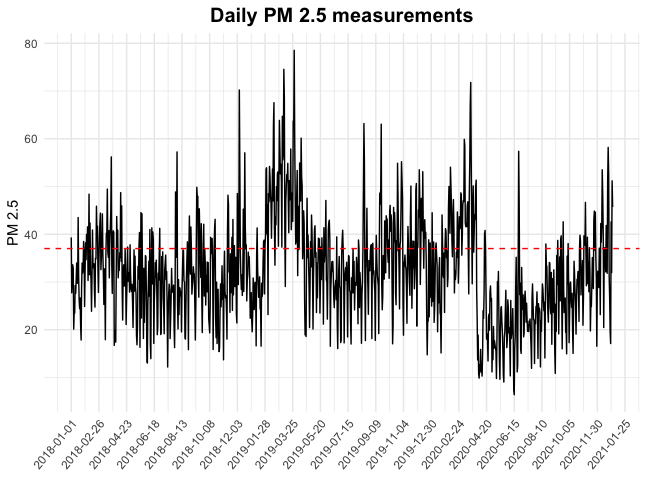
\includegraphics[width=09cm]{PM25.png}
\caption{PM 2.5 Measurements in Bogota, January 1 2018 - December 21 2020}
\label{fig:Daily}
\end{center}
\end{figure}

The conditions considered in the present implementation included taking generations of size 50 with 50 offspring each. The distributions used to generate the first generation and the mutations were those mentioned in section (\ref{Genetic Algorithm Scheme}).As initial settings for the values to be optimized in the first equation of expression (\ref{eq1}), $\alpha$ and $\beta$ are 0.1 and 0.5 respectively. For this optimization process we made use of the R optim library.

The a-priori distributions used for the parameters $\alpha$ and $\beta$ are Gammas with hyperparameters $\phi_{11}= 1, \phi_{12} = 2, \phi_{21} = 3$ and $\phi_{22}= 1.2$, as defined in section (\ref{Weibull}), given that the intensity rate in use is Weibull.

The optimal chromosome was found to be (8, 400, 408, 445, 488, 627, 654661, 798), where it is indicated that there are 8 points of change, followed by their respective location in the 1096 days of the observed timeline, and the first 4 change points are very close. Their corresponding MDL value was 743.0601. The following table (\ref{table:Points}) shows the date corresponding to each change point.


\begin{table}[h]
\begin{center}
\begin{tabular}{c|c|c}
\textbf{Change Point} & \textbf{Day of the week} & \textbf{Date}      \\ \hline
400                   & Monday                   & February 4, 2019   \\
408                   & Tuesday                  & February 12, 2019  \\
445                   & Thursday                 & March 21, 2019     \\
488                   & Friday                   & May 3, 2019        \\
627                   & Thursday                 & September 19, 2019 \\
654                   & Wednesday                & October 16, 2019   \\
661                   & Wednesday                & October 23, 2019   \\
798                   & Sunday                   & March 8, 2020     
\end{tabular}
\end{center}
\caption{Points of change and their respective dates}
\label{table:Points}
\end{table}


The months in which these surpasses occur are during the rainy season in Bogota. If the dates in the table above are compared with the measurements in Figure (1), the seasons with the most consistent peaks over time can be captured.

As can be seen in the graphs in figure (\ref{fig:fig2}), in the upper left graph is found the adjustment of the cumulative mean function $m(t|\theta)$ (black line), by means of the point averages obtained by the vectors of parameters better qualified by the MDL (red line) and their respective 95\% confidence intervals (blue lines).

In the upper right graph is the evaluation by MDL of each of the best chromosomes of each of the 50 generations, in which case it is observed that the one with the lowest one is the member of generation 24, which has 8 points of change. In the lower left graph, the histogram shows the days in the time series that exceed the threshold, which appear most frequently in the first 50 chromosomes of the 50 generations analyzed.


\begin{figure}[h]
\begin{center}
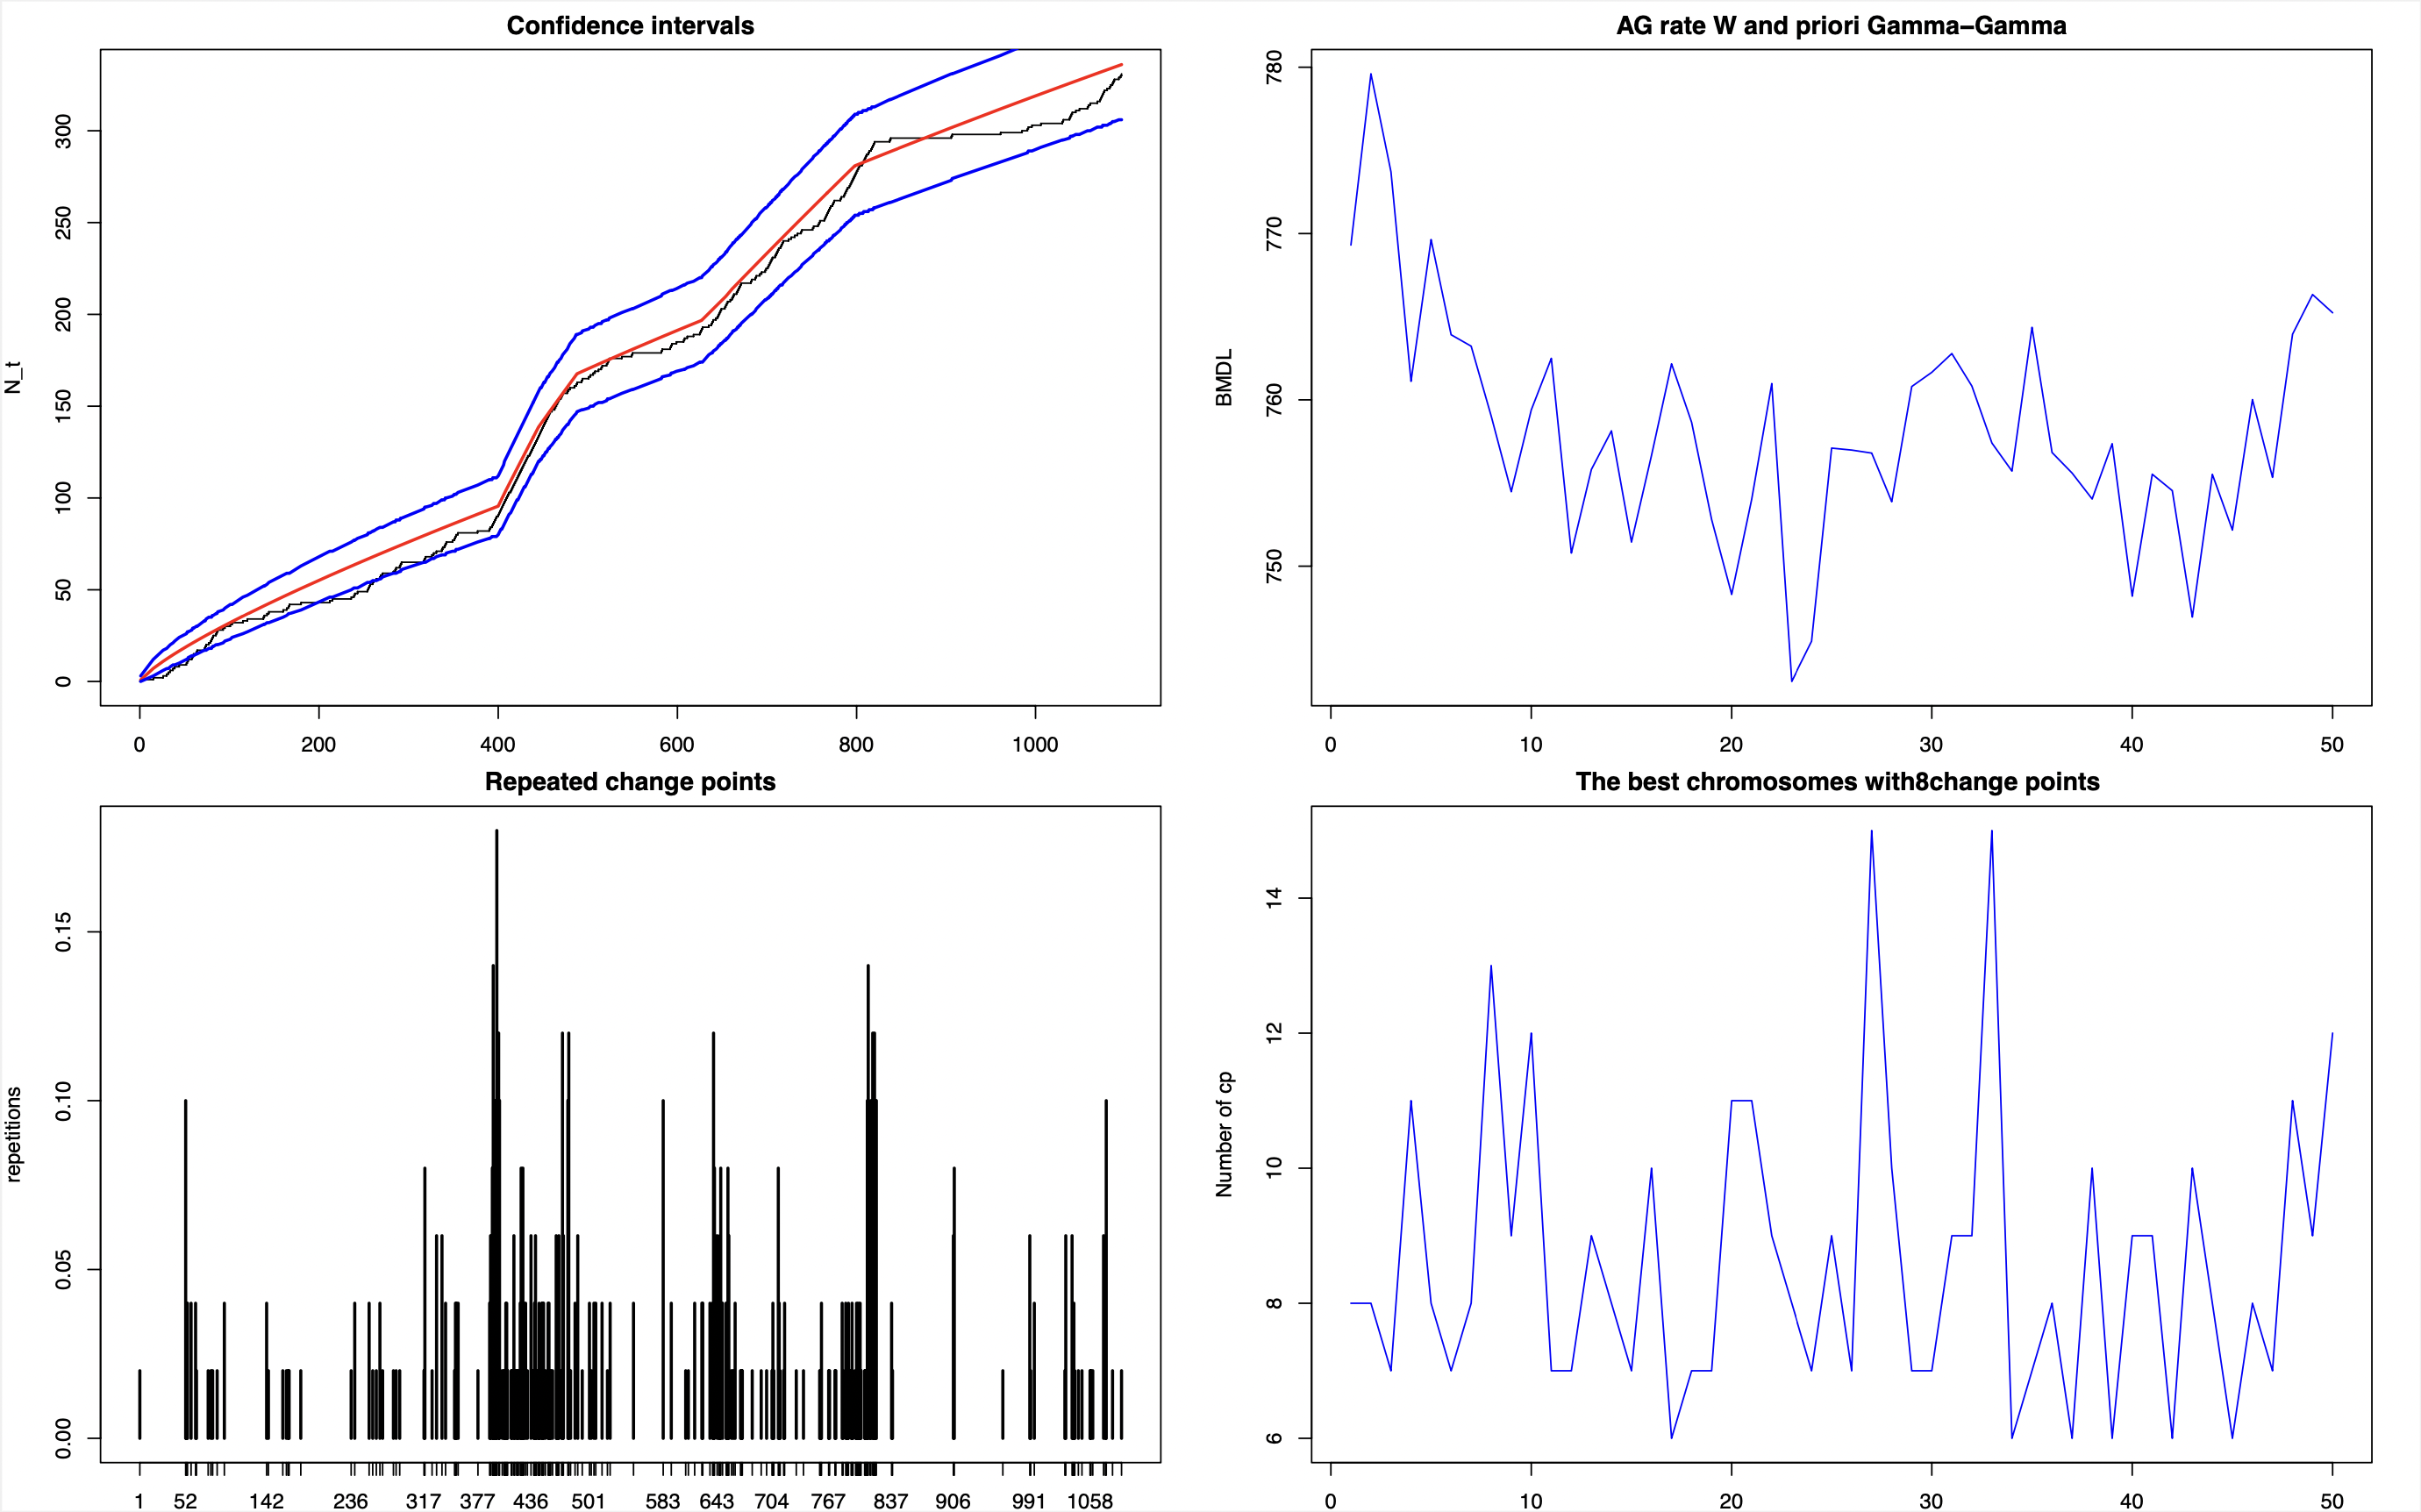
\includegraphics[width=16cm]{Fourgraph.png}
\end{center}
\caption{Results for the Optimal Chromosome}
\label{fig:fig2}
\end{figure}




The graph in figure (\ref{fig:fig3}) shows that before day 400, i.e., Monday, February 4, the rate of exceedances of the 37 $\mu$g/$m^3$ threshold had been decreasing sharply, after which, for eight consecutive days, it recorded the highest emission rate. This high average rate is around 1.004, as shown in Table (\ref{table:Regime}) for the second regime. In the third regime it decreased to an average rate of 0.9468, in the fourth it jumps to 0.6748 and it is in the fifth regime that it achieves the lowest drop (0.2090), before the intensity function rises again to levels above 0.2 threshold overshoots per unit of time. This  rate present in the fifth regime has cut-off dates of May 3 to September 19, 2019. Thus, it is evident that the fifth regime occurs before the Pandemic quarantine was declared in Colombia, therefore, this may be the result of public policy aimed at reducing the emission of PM2.5.


\begin{figure}[h]
\begin{center}
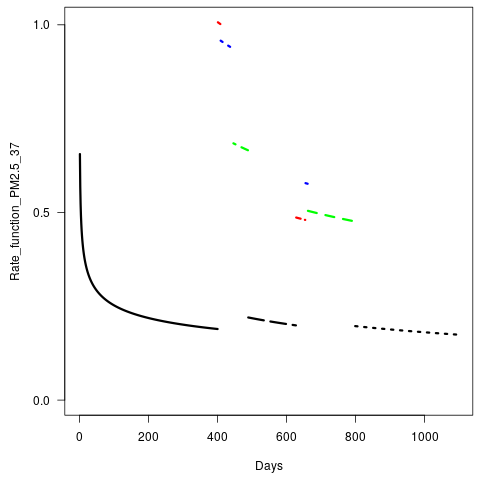
\includegraphics[width=10cm]{funcion de riesgo.png}
\end{center}
\caption{Rate function for PM 2.5 by Days}
\label{fig:fig3}
\end{figure}



In terms of public policy, three major projects were implemented as part of the 2010-2020 ten-year plan for air pollution control: The use of emission control systems in cargo transport vehicles and motorcycles, as well as the SITP integrated public transport system. The later includes the replacement of old buses with internal combustion engine by electric or hybrid buses. In addition to the above, a few days before the fifth regime, resolution 383 (see RES19 (2019)) is issued, which declares a yellow alert for particulate matter exceedances. Considering the first regime represented in figure (\ref{fig:fig3}), its rapid deceleration in the emission of threshold exceedances can also be seen as a consequence of these resolution , in which the yellow alert for environmental pollution is decreed and some restrictions are established in the city of Bogota. Such is the case of restrictions in the transportation and mobility sector, in addition to those established for the operations of industrial sources that use combustion processes associated mainly with the burning of biomass, use of fossil or liquid fuels.

\begin{table}[h]
\begin{center}
\begin{tabular}{c|c|c|c}
\textbf{Regime} & \textbf{Min} & \textbf{Mean} & \textbf{Max} \\ \hline
1               & 0.1894       & 0.2379        & 0.6555       \\
2               & 1.002        & 1.004         & 1.007        \\
3               & 0.9363       & 0.9468        & 0.9577       \\
4               & 0.6657       & 0.6748        & 0.6841       \\
5               & 0.1991       & 0.2090        & 0.2201       \\
6               & 0.4801       & 0.4832        & 0.4864       \\
7               & 0.5765       & 0.5773        & 0.5781       \\
8               & 0.4761       & 0.4896        & 0.5043       \\
9               & 0.1744       & 0.1849        & 0.1971      
\end{tabular}
\end{center}
\caption{Minimum, Maximum and Mean for each Regime}
\label{table:Regime}
\end{table}



\section{Conclussions and future work}\label{sec9}

The method of detection of change points from the genetic algorithm and using MDL as selection criteria yielded results that agree with the public policies implemented in Bogota, both regarding the contamination alerts issued by the monitoring network, as well as the mobility restrictions due to the quarantine caused by the SARS-CoV-2 virus pandemic.  It is seen that the model gives good results both in regions with stations, the case of Mexico City, (\cite{Achcar10}, \cite{Achcar11})and in tropical areas where these periodic temperature changes do not occur, showing the robustness of the technique. We hope that in the near future these methods will prove to be a tool used by the agents in charge of measuring the effectiveness of the actions taken to reduce air pollution and thus reduce its impacts both on the environment and on the health of the inhabitants.




\bibliography{wileyNJD-APA}



\end{document}

